\documentclass[conference]{IEEEtran}
\IEEEoverridecommandlockouts
% The preceding line is only needed to identify funding in the first footnote. If that is unneeded, please comment it out.
\usepackage{cite}
\usepackage{amsmath,amssymb,amsfonts}
\usepackage{algorithmic}
\usepackage{graphicx}
\usepackage{textcomp}
\usepackage{xcolor}

\usepackage{physics}
\usepackage{amsmath}
\usepackage{tikz}
\usepackage{mathdots}
\usepackage{yhmath}
\usepackage{cancel}
\usepackage{color}
\usepackage{siunitx}
\usepackage{array}
\usepackage{multirow}
\usepackage{amssymb}
\usepackage{gensymb}
\usepackage{tabularx}
\usepackage{extarrows}
\usepackage{booktabs}
\usetikzlibrary{fadings}
\usetikzlibrary{patterns}
\usetikzlibrary{shadows.blur}
\usetikzlibrary{shapes}
\usepackage[figure]{ragged2e}

\usepackage{graphicx}
\usepackage{caption}
\usepackage{subcaption}





\def\BibTeX{{\rm B\kern-.05em{\sc i\kern-.025em b}\kern-.08em
    T\kern-.1667em\lower.7ex\hbox{E}\kern-.125emX}}
\begin{document}

\title{Design of an Autonomous Temperature Conditioning System Using Modified PID Controller\\
{}
}

\author{\IEEEauthorblockN{Özgür Gülsuna}
\IEEEauthorblockA{\textit{Electrical and Electronics Engineering} \\
\textit{Middle East Technical University}\\
Ankara, Turkey \\}
\and
\IEEEauthorblockN{Işık Emir Altunkol}
\IEEEauthorblockA{\textit{Electrical and Electronics Engineering} \\
\textit{Middle East Technical University}\\
Ankara, Turkey \\}
}

\maketitle

\begin{abstract}
Designing a responsive, fast, and accurate temperature conditioning system is not a simple challenge due to the complexity of thermal systems and the asymmetry between the heating and cooling operations. This report focuses on the design, simulation and prototyping of an autonomous temperature conditioning system using a modified PID (Proportional Integral Derivative) method. The system is heated with a resistive heater and cooled with a fan. In order to achieve a fast, responsive and accurate control, PID control method, which is widely used in industry, is utilized. The asymmetry of the heating and cooling systems bring an accuracy problem. The proposed solution is to modify the standard PID configuration in a specific manner. The temperature is measured with LM35 analog temperature sensor. Both the set and ambient temperatures are displayed using RGB (Red Green Blue) LEDs (Light Emitting Diodes) with a continuous color transmission from blue to green and green to red as the temperature increases. The circuit is constructed on a PCB (Printed Circuit Board), which reduced the EMI (Electromagnetic Interference) problems distorting the critical control signals. The stackable structure is used to make the system more compact, rigid, and easy to use. A thermal model is constructed to simulate the system realistically. Finally, a comparison of experimental results with the simulation results is presented.
\end{abstract}

\begin{IEEEkeywords}
temperature control, asymmetric PID, thermal modelling
\end{IEEEkeywords}

\section{Introduction}
In the industry, various control techniques are used for automating the physical processes. One of the simplest one is the on-off control, in which the operating unit is either actuated or not depending on other system and state parameters. However, the on-off control method is not flexible and accurate for most of the control problems. Because of that a slightly more advanced method called PID (Proportional Integral Derivative) is widely utilized in industry.



\begin{figure}[ht]
\centerline{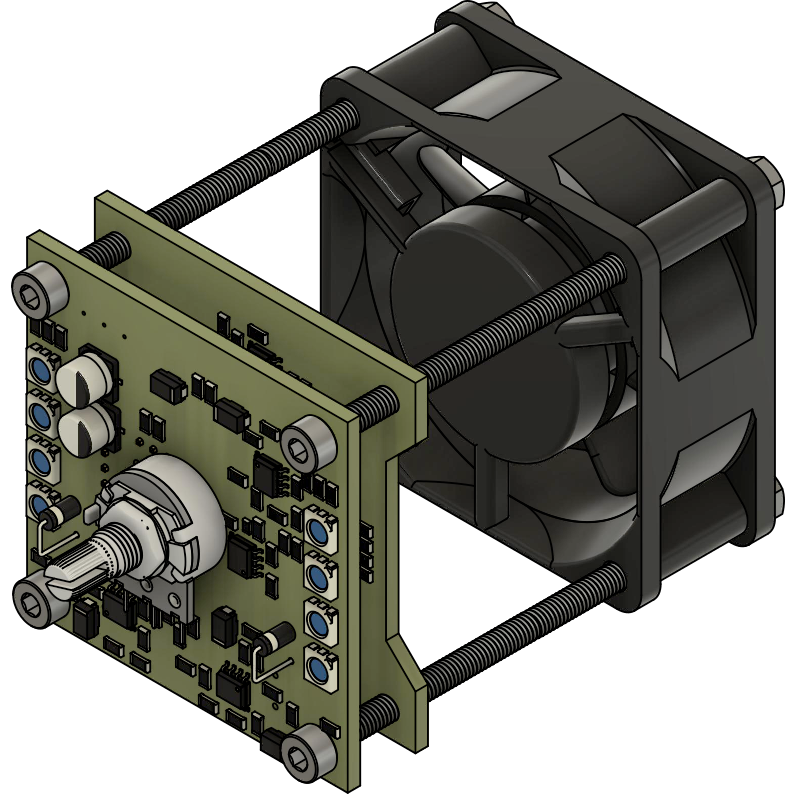
\includegraphics[scale=0.28]{figures/model2.png}}
\caption{Computer aided drawing of the presented system.}
\label{}
\end{figure}



Thus to design a responsive, fast, and accurate temperature control system PID method is a feasible choice. One challenge of applying PID method to this problem is that the heating and cooling processes are not symmetric. To compensate that, a modified PID control circuit will be introduced in this paper. Also, to avoid the EMI (Electromagnetic Interference) and noise problems, the circuit is designed on a PCB (Printed Circuit Board).

The heating element is a nickel-chromium wire and the cooling element is an 12V DC fan. The fan and the heater are driven with a MOSFET switch which is controlled by the generated PWM (Pulse Width Modulation) signals. The PWM for each switch is generated by comparing a triangular wave with the PID outputs.

The ambient temperature is measured using the LM35 analog temperature sensor. The set temperature value is adjusted with a potentiometer. The set and ambient temperatures are displayed by the display unit which consist of RGB LEDs (Red Green Blue Light Emitting Diodes), a constant current LED drive utilized by a transconductance amplifier. The display unit designed in a way to emit red light at 24\celsius and below, green light at 32\celsius and blue light at 40\celsius and above. The display output for the temperature intervals between those values are produced by combining the colors in a way that a smooth transition is observed while the set and ambient temperatures are changed.

In this paper, first the design methodology and the mathematical analysis of each unit will be discussed in detail in section II. The circuit schematics and their analysis will be given in this part. The mechanical design and the manufacturing will be discussed in section III. Then, thermal modelling of the system will be explained in section IV. The results of the performed LTspice simulations will be given in section V. The experimental results and the comparison with the simulation will follow in section VI. Finally, the conclusions will be drawn in section VII.


\section{Design Methodology and Mathematical Analysis}

In this section the design criteria are analyzed and solutions to each unit is presented with mathematical analysis of circuits are explained in detail.
 
\subsection{Sensing Unit}

The sensing unit consists of two independent sub-sections as mentioned above. The first element is the LM35 temperature sensor. This sensor gives a linear analog voltage output between -55$ ^\circ$C and 150  $ ^\circ$C in consequence it is applicable for the designs needs. The output of this sensor is amplified to ten folds such that 28$^\circ$C is scaled as 2.8 volts. This primary amplification facilitates the signal in order to better process it in the later stages. The second element is a potentiometer, which is basically a reference input and it is used in an adjustable resistor division configuration which scales the position to the range between 2 volts and 4.5 volts to cover the operation range of 20 to 45 $^\circ$C.

As in most of the sensory data acquisition, an initial low pass filter is used to clear out the unwanted high-frequency signals\cite{b1}. The design for this initial unit has an R-C low pass filter with the cut off frequency of 338.6 Hz \eqref{filter} which is selected as it is around 1/3 of the switching frequency of the operation unit. 
\begin{equation*}
f_{cut-off} =\frac{1}{2\pi RC} \rightarrow 338.6\ Hz \label{filter}
\end{equation*}

Another feature this section has is a linear regulator to supply the LM35 sensor. The selected voltage regulator is LM7805 which is a linear type and it is used to isolate the input of the temperature sensor from the unwanted swing of the input voltage.

\begin{figure}[h]
\centerline{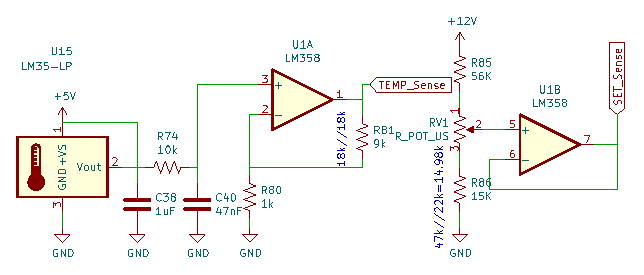
\includegraphics[scale=0.75]{figures/sense-sch.eps}}
\caption{Circuit schematic of the sensing unit}
\label{fig}
\end{figure}

The outputs of this unit are forwarded to the display and control units.

\subsection{Display Unit}

The display unit takes two inputs from the sensing unit: one is the amplified ambient temperature signal and the other is the set value, which is scaled to the same range with the temperature signal. This unit produces three different voltage signals to drive the RGB LEDs (one for each color), both for the set value display and the ambient temperature display. Since LED brightness is linearly proportional with its current, a transconductance amplifier with a BJT (Bipolar Junction Transistor) is used as a constant current LED driver (Fig.~\ref{transcondAmp}). Assuming the BJT is in forward active operation:



\begin{figure}[h]
\centerline{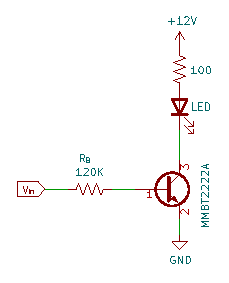
\includegraphics[scale=1]{figures/transcond-amp.eps}}
\caption{Transconductance amplifier as a constant current driver}
\label{transcondAmp}
\end{figure}

\begin{equation}
I_{C} = \beta \times \frac{V_{in}-V_{BE_{on}}}{R_{B}}\label{Iled}
\end{equation}


By \eqref{Iled}, it is observed that the input voltage signal is shifted downwards by $V_{BE_{on}}$ and then amplified by $\frac{\beta}{R_{B}}$. The collector current needed for the corresponding amplifier to obtain the required brightness for each color terminal is given in Fig.~\ref{ILED}.

\begin{figure}[h]
\centerline{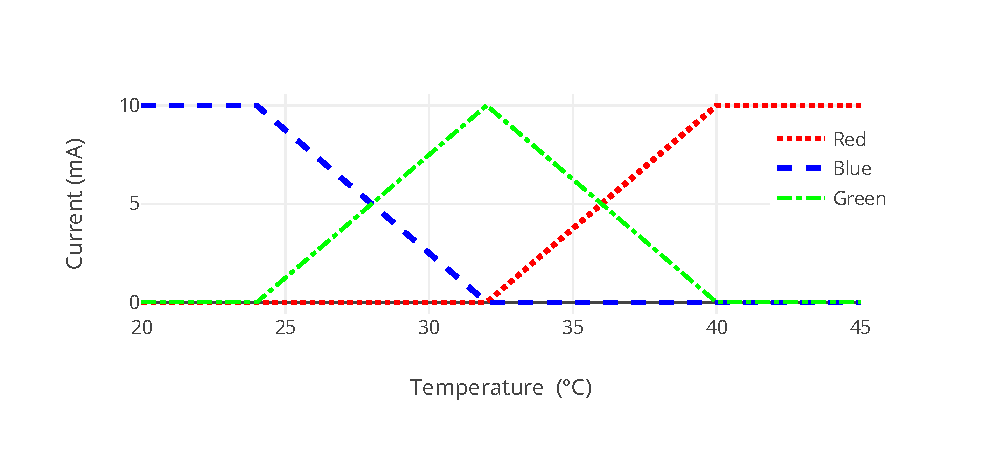
\includegraphics[scale=0.58]{figures/current_vs_temp.eps}}
\vspace{-1em}
\caption{Current vs temperature for each color terminal}
\label{ILED}
\end{figure}

To obtain the current signal in Fig.~\ref{ILED}, the voltage $V_{in}$ must be in the same shape, but shifted up by $V_{BE_{on}}$. This is why there is an amplifier stage which adds the diode drop value to the amplified set and temperature voltages. The schematic of these amplifiers is given in figure Fig.~\ref{dropSubtracter}. It can be easily observed that the input output relation for the amplifiers in figure Fig.~\ref{dropSubtracter} is given as:

\begin{equation}
V_{1}' = 2\cdot V_{1}+V_{BE_{on}}\label{drop_sub}
\end{equation}

\begin{figure}[h]
\centerline{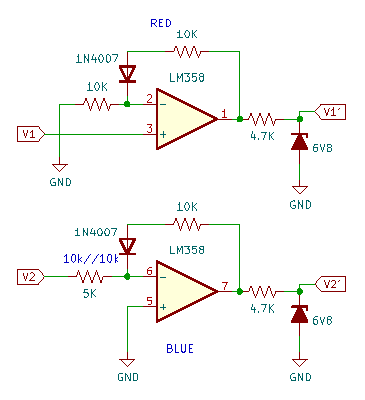
\includegraphics[scale=1.0]{figures/display-diode-drop-subtractor.eps}}
\caption{Circuit schematic for $V_{BE_{on}}$ compensator}
\label{dropSubtracter}
\end{figure}

Note that the diode drop and the base emitter voltage drop of the transistors are approximately equal, since they are both made of silicon. The zener diode connected in shunt clips the voltage above 6.8V, which creates an upper limit for input voltage of the transconductance amplifier. Considering these, the process for obtaining the red and blue LED currents is the following: An offset is added to the temperature signal (or the set value signal, for the set display) to align its 0 value to the center of the operation region of the circuit (32\celsius). Then, this new signal is connected to $V_{1}$ \& $V_{2}$ terminals of the amplifier in figure Fig.~\ref{dropSubtracter}. Finally, determining $R_{C}=120k\Omega$ and connecting the output of the compensator to the input of the transconductance amplifier, we obtain the desired current signal.

A straightforward way to obtain the green LED current is to use an inverting summing amplifier and sum the voltage signals produced at the outputs of the figure Fig.~\ref{dropSubtracter}, and transmit this sum to the input of the transconductance amplifier. Note that the inverting sum result is a shifted version of the desired voltage, therefore the appropriate offset should be applied during the summing operation. Connecting all of the aforementioned parts, a display unit with a smooth and precise output is designed.


\subsection{Control Unit}
One of the more ingenious ways of controlling a dynamic system is PID method. This three-term controller is commonly used in the industry because of its accuracy and responsiveness \cite{b2}. Therefore it is selected as the main controller, more precisely a version with parallel configuration of action parameters of PID is selected. This approach isolates the parameters from each other which provides an easier tuning procedure for our system.









The system has two process variables in other words two outputs that can be controlled with our controller. These two actuators, heating element and fan, are working asynchronous with opposite reactions. This duality enforces an asymmetry in our system and it should be addressed to improve the response of the system \cite{b3}. The first solution comes in mind is to separate the controllers for each process variable but it increases the cost both in terms of components and tuning time. Our proposed method utilizes a single PID controller for the heater and its output is passed through a proportional term which then it is fed to the fan. This cascaded configuration presented in Fig.~\ref{parallelPID} enables the system to utilize its integral and derivative terms in both of the outputs. 



\begin{figure}[h]




\tikzset{every picture/.style={line width=0.75pt}} %set default line width to 0.75pt        

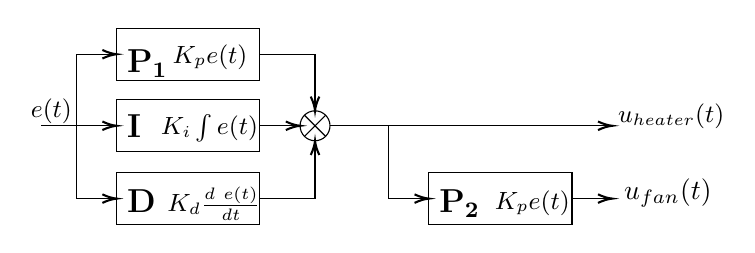
\begin{tikzpicture}[x=0.47pt,y=0.47pt,yscale=-1,xscale=1]
%uncomment if require: \path (0,235); %set diagram left start at 0, and has height of 235

%Shape: Resistor [id:dp04371691643945974] 
\draw   (135.96,39) -- (246.04,39) -- (246.04,79) -- (135.96,79) -- (135.96,39) -- cycle (105,59) -- (135.96,59) (246.04,59) -- (277,59) ;
%Shape: Resistor [id:dp10680848125616538] 
\draw   (135.96,94) -- (246.04,94) -- (246.04,134) -- (135.96,134) -- (135.96,94) -- cycle (105,114) -- (135.96,114) (246.04,114) -- (277,114) ;
%Shape: Resistor [id:dp6702844773190892] 
\draw   (135.96,150) -- (246.04,150) -- (246.04,190) -- (135.96,190) -- (135.96,150) -- cycle (105,170) -- (135.96,170) (246.04,170) -- (277,170) ;
%Straight Lines [id:da9493111687595024] 
\draw    (105,59) -- (105,170) ;
%Straight Lines [id:da22129182527616287] 
\draw    (105,59) -- (133.96,59) ;
\draw [shift={(135.96,59)}, rotate = 180] [color={rgb, 255:red, 0; green, 0; blue, 0 }  ][line width=0.75]    (10.93,-3.29) .. controls (6.95,-1.4) and (3.31,-0.3) .. (0,0) .. controls (3.31,0.3) and (6.95,1.4) .. (10.93,3.29)   ;
%Straight Lines [id:da46981664928370725] 
\draw    (105,114) -- (133.96,114) ;
\draw [shift={(135.96,114)}, rotate = 180] [color={rgb, 255:red, 0; green, 0; blue, 0 }  ][line width=0.75]    (10.93,-3.29) .. controls (6.95,-1.4) and (3.31,-0.3) .. (0,0) .. controls (3.31,0.3) and (6.95,1.4) .. (10.93,3.29)   ;
%Straight Lines [id:da05179885664599704] 
\draw    (105,170) -- (133.96,170) ;
\draw [shift={(135.96,170)}, rotate = 180] [color={rgb, 255:red, 0; green, 0; blue, 0 }  ][line width=0.75]    (10.93,-3.29) .. controls (6.95,-1.4) and (3.31,-0.3) .. (0,0) .. controls (3.31,0.3) and (6.95,1.4) .. (10.93,3.29)   ;
%Straight Lines [id:da6012096316257116] 
\draw    (246.04,114) -- (275,114) ;
\draw [shift={(277,114)}, rotate = 180] [color={rgb, 255:red, 0; green, 0; blue, 0 }  ][line width=0.75]    (10.93,-3.29) .. controls (6.95,-1.4) and (3.31,-0.3) .. (0,0) .. controls (3.31,0.3) and (6.95,1.4) .. (10.93,3.29)   ;
%Straight Lines [id:da20403881397537615] 
\draw    (288.5,170) -- (288.5,127.5) ;
\draw [shift={(288.5,125.5)}, rotate = 90] [color={rgb, 255:red, 0; green, 0; blue, 0 }  ][line width=0.75]    (10.93,-3.29) .. controls (6.95,-1.4) and (3.31,-0.3) .. (0,0) .. controls (3.31,0.3) and (6.95,1.4) .. (10.93,3.29)   ;
%Straight Lines [id:da27228914592677467] 
\draw    (288.5,59) -- (288.5,100.5) ;
\draw [shift={(288.5,102.5)}, rotate = 270] [color={rgb, 255:red, 0; green, 0; blue, 0 }  ][line width=0.75]    (10.93,-3.29) .. controls (6.95,-1.4) and (3.31,-0.3) .. (0,0) .. controls (3.31,0.3) and (6.95,1.4) .. (10.93,3.29)   ;
%Flowchart: Summing Junction [id:dp5290671545073427] 
\draw   (277,114) .. controls (277,107.65) and (282.15,102.5) .. (288.5,102.5) .. controls (294.85,102.5) and (300,107.65) .. (300,114) .. controls (300,120.35) and (294.85,125.5) .. (288.5,125.5) .. controls (282.15,125.5) and (277,120.35) .. (277,114) -- cycle ; \draw   (280.37,105.87) -- (296.63,122.13) ; \draw   (296.63,105.87) -- (280.37,122.13) ;
%Straight Lines [id:da746161281015258] 
\draw    (277,170) -- (288.5,170) ;
%Straight Lines [id:da11789860127120222] 
\draw    (277,59) -- (288.5,59) ;
%Straight Lines [id:da810785702729852] 
\draw    (78,114) -- (105,114) ;
%Straight Lines [id:da03181312676625048] 
\draw    (300,114) -- (510,114) ;
%Shape: Resistor [id:dp25780959233444034] 
\draw   (375.96,150) -- (486.04,150) -- (486.04,190) -- (375.96,190) -- (375.96,150) -- cycle (345,170) -- (375.96,170) (486.04,170) -- (517,170) ;
%Straight Lines [id:da21977667644036813] 
\draw    (345,170) -- (373.96,170) ;
\draw [shift={(375.96,170)}, rotate = 180] [color={rgb, 255:red, 0; green, 0; blue, 0 }  ][line width=0.75]    (10.93,-3.29) .. controls (6.95,-1.4) and (3.31,-0.3) .. (0,0) .. controls (3.31,0.3) and (6.95,1.4) .. (10.93,3.29)   ;
%Straight Lines [id:da016506681158132253] 
\draw    (345,170) -- (345,113.67) ;
%Straight Lines [id:da8718572314475974] 
\draw    (486.04,170) -- (515,170) ;
\draw [shift={(517,170)}, rotate = 180] [color={rgb, 255:red, 0; green, 0; blue, 0 }  ][line width=0.75]    (10.93,-3.29) .. controls (6.95,-1.4) and (3.31,-0.3) .. (0,0) .. controls (3.31,0.3) and (6.95,1.4) .. (10.93,3.29)   ;
%Straight Lines [id:da33938783257620053] 
\draw    (300,114) -- (515,114) ;
\draw [shift={(517,114)}, rotate = 180] [color={rgb, 255:red, 0; green, 0; blue, 0 }  ][line width=0.75]    (10.93,-3.29) .. controls (6.95,-1.4) and (3.31,-0.3) .. (0,0) .. controls (3.31,0.3) and (6.95,1.4) .. (10.93,3.29)   ;

% Text Node
\draw (177,49.4) node [anchor=north west][inner sep=0.75pt]  [font=\small]   {$K_{p} e( t)$};
% Text Node
\draw (168,103.4) node [anchor=north west][inner sep=0.75pt]  [font=\small]     {${\textstyle K_{i}\int e( t)}$};
% Text Node
\draw (173,159.4) node [anchor=north west][inner sep=0.75pt]   [font=\small]    {${\textstyle K_{d}\frac{d\ e( t)}{dt}}$};
% Text Node
\draw (68,91.4) node [anchor=north west][inner sep=0.75pt]   [font=\small]    {$e( t)$};
% Text Node
\draw (519.49,95.4) node [anchor=north west][inner sep=0.75pt]   [font=\small]    {$u_{heater}( t)$};
% Text Node
\draw (424.82,161.73) node [anchor=north west][inner sep=0.75pt]   [font=\small]    {$K_{p} e( t)$};
% Text Node
\draw (142,53.4) node [anchor=north west][inner sep=0.75pt]  [font=\large]  {${\displaystyle \mathbf{P}_{\mathbf{1}}}$};
% Text Node
\draw (142,103.4) node [anchor=north west][inner sep=0.75pt]  [font=\large]  {$\mathbf{I}$};
% Text Node
\draw (142,161.4) node [anchor=north west][inner sep=0.75pt]  [font=\large]  {$\mathbf{D}$};
% Text Node
\draw (382,161.4) node [anchor=north west][inner sep=0.75pt]  [font=\large]  {${\displaystyle \mathbf{P}_{\mathbf{2}}}$};
% Text Node
\draw (524.16,152.73) node [anchor=north west][inner sep=0.75pt]    {$u_{fan}( t)$};


\end{tikzpicture}


\caption{Proposed modified PID controller block diagram.}
\label{parallelPID}
\end{figure}




The controller in this section is implemented using operational amplifiers in an analogous way. First the error is generated using non inverting difference amplifier with unity gain. The error is then passed to three parallel stages which are proportional, integral and derivative terms. These configurations are inverting amplifiers by nature. Then the inverting summing amplifier is used to sum the action parameters into one. The circuit diagram of the control unit can be seen in Fig.~\ref{PIDcct}.



\begin{figure}[h]
    \centering
    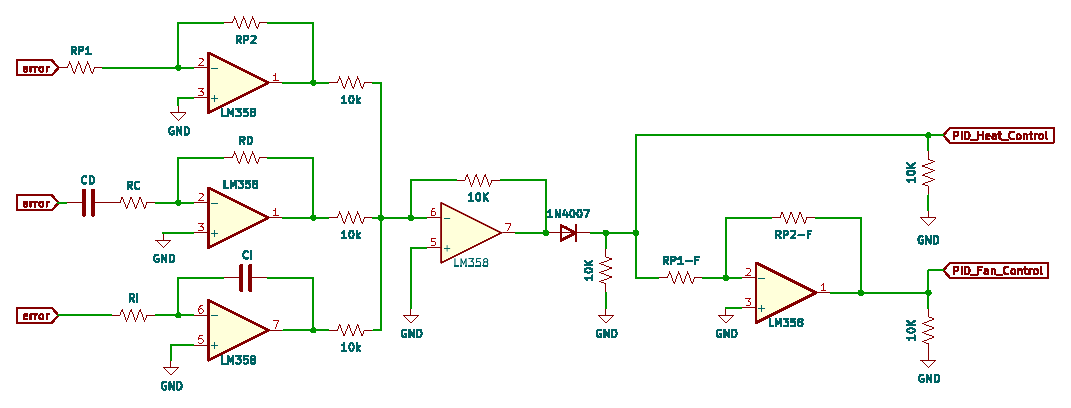
\includegraphics[scale=0.5]{figures/PID.eps}
    \caption{PID implementation using operational amplifiers}
    \label{PIDcct}
\end{figure}





Key point of the control unit is the derivative term. Differentiator amplifier circuit acts as a high pass filter, in other words it enables high frequency components of the input signal to not only to pass but to be amplified \cite{b4}. It is an undesired condition since our switching frequency is around 1 kHz and it is easily coupled into the error signal. Amplifying this noise signal can cause the control signal to become erratic. Analyzing the differentiator circuit given in Fig.~\ref{diffe} shows this phenomena more clearly.


\begin{figure}[h]
    \centering
    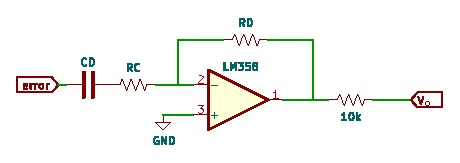
\includegraphics[scale=1]{figures/derivative.eps}
    \caption{Differentiator circuit to be analyzed.}
    \label{diffe}
\end{figure}





As seen in \eqref{derform} for high frequencies impedance of the capacitor is very small and in absence of $R_C$ resistor the gain is very high. In order to limit this gain a resistor of 1 k$\Omega$ is selected. 


\begin{equation}
V_{out} =\frac{-V_{error}R_D}{R_C + \frac{1}{sC_D}}\label{derform}
\end{equation}






\subsection{Operation Unit}

The purpose of the operation unit is to take the PID output signals from the control unit and produce PWM signals to drive the heater and the fan using a switch. The PWM method is utilized to convert the analog signals of the control unit into digital signals that can drive the MOSFETs. 

The first stage is a triangular wave generator (Fig.~\ref{triGen}). The left part in Fig.~\ref{triGen} is an astable multivibrator, which creates a square wave with the frequency given as:

\begin{equation}
f=\frac{1}{2R_{1}C_{1}\ln{(1+\frac{2R_{3}}{R_{2}})}}\label{freq}
\end{equation}

\begin{figure}[h]
\centerline{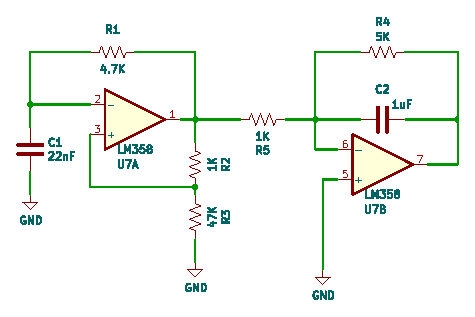
\includegraphics[scale=1]{figures/osci.eps}}
\caption{Circuit schematic of the triangular wave generator}
\label{triGen}
\end{figure}

Since it is aimed to achieve a PWM frequency around $1kHz$, the component values are chosen as $R_{1}=4.7k\Omega, C_{1}=22nF, R_{2}=1k\Omega, R_{3}=47k\Omega$ which brings $1.062kHz$ by \eqref{freq}. The multivibrator output is given to the integrator circuit, whose time constant is chosen as $R_{4}C_{2}=5ms$. Thus, $0.2$ time constant of the exponential waveform is produced, which is close enough to a triangular wave. After adding an offset and amplifying to an appropriate range, the triangular wave is supplied to two comparators to generate the PWM signals. The minimum points of the final triangular wave is higher than 0 volts by a couple hundred mVs, so that the heather or the fan does not act even for small disturbances in the control signals.

The PWM generating process for the heater is done in the conventional way. The triangular wave is compared with the PID heater output signal, and then a MOSFET is used as a switch to drive the heater with the PWM signal. The same process is applied to for the fan, except that after the cooperator, an additional compactor step is added to avoid powering the fan while the heater operates (Fig.~\ref{fanAND}). The second op-amp stage checks if the PID heater output is still higher than a certain threshold voltage (which is a positive value close to 0), and turns the switch on only if it is smaller than the threshold voltage. In this way, our design criteria is satisfied.

\begin{figure}[h]
\centerline{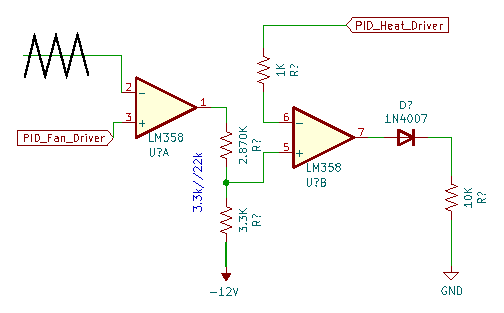
\includegraphics[scale=1]{figures/COMP.eps}}
\caption{Circuit schematic of the comparators}
\label{fanAND}
\end{figure}

While the heater operates, the maximum power consumed by the system is less than 12W.

\section{Mechanical Design and Manufacturing}
Design of the mechanical system is formed around the biggest component which is the fan. It is 60x60 mm in width and 25 mm in depth with four bolt holes on four corners. These holes are used with 3mm bolts to construct a frame around the fan and circuit elements. These elements consist of operational amplifiers, LEDs, passive components such as resistors and capacitors and heater with the temperature sensor. All elements are fixed on printed circuit board (PCB) besides the fan. To satisfy the small form factor criteria PCB dimensions are selected again 60x60 mm and surface mount components are used. 

Heater element is a nickel-chromium wire which is used in electric heaters.The wire is wrapped into a spring shape and formed into a circle around the temperature sensor.This element has advantages such as enduring high temperatures, having a relatively high resistance which makes it smaller and being malleable. 

The power connector has three pins 12V, ground and -12V respectively. It connects only one way which makes it more convenient.

PCB is designed to form the circuit on. This technology has two advantages on analog circuits. The first one is with careful track planning noise susceptibility is reduced. The parasitic resistances, inductances and capacitances are also minimized. The second advantage is its rigidity and compactness. Design of the PCB is done on KiCad which is an open-source circuit board drawing program. The design consist two double-sided boards with connectors in-between. This stackable composition has advantages in both initial testing of the boards and in isolating the power paths from signal paths. The more outer board consist of sensing unit, display unit and control unit. All of these units consume very little power and they produce the control signals. The second board only has the operation unit. The most of the power is directed through this board. The PWM method creates changing currents and when we look at the equation of induced voltage in \eqref{indVolt}. It can be observed that time altering magnetic field generated from AC currents of the PWM signals, induces emf voltage on the magnetically coupled regions of the circuit. This way the noise is transmitted on signal paths. 

\begin{equation}
V_{ind} = L\frac{di}{dt} \label{indVolt}    
\end{equation}

Separating the boards reduces this interference and effectively isolates the signal paths. 

Input bus capacitors and decoupling capacitors near the operational amplifiers are working in a similar manner. These components filter out the noise from the input source and reduce the conducted EMI (Electromagnetic Interference) between sections.


\begin{figure}[!tbp]
  \begin{subfigure}[b]{0.319\textwidth}
    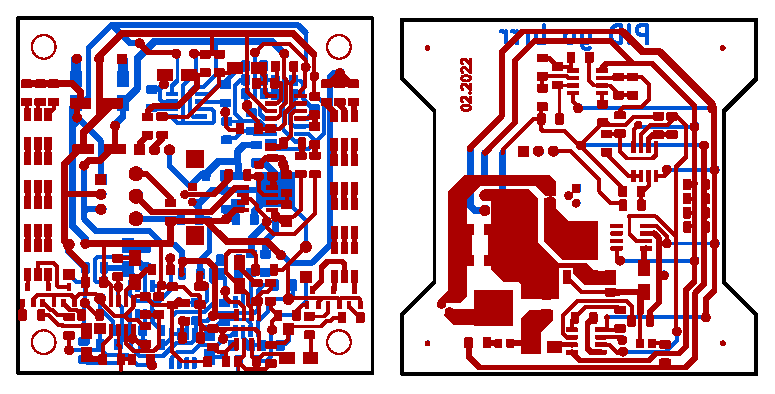
\includegraphics[width=\textwidth]{figures/pcb.eps}
    \caption{print out of the design.}
    \label{PCB}
  \end{subfigure}
  \hfill
  \begin{subfigure}[b]{0.158\textwidth}
    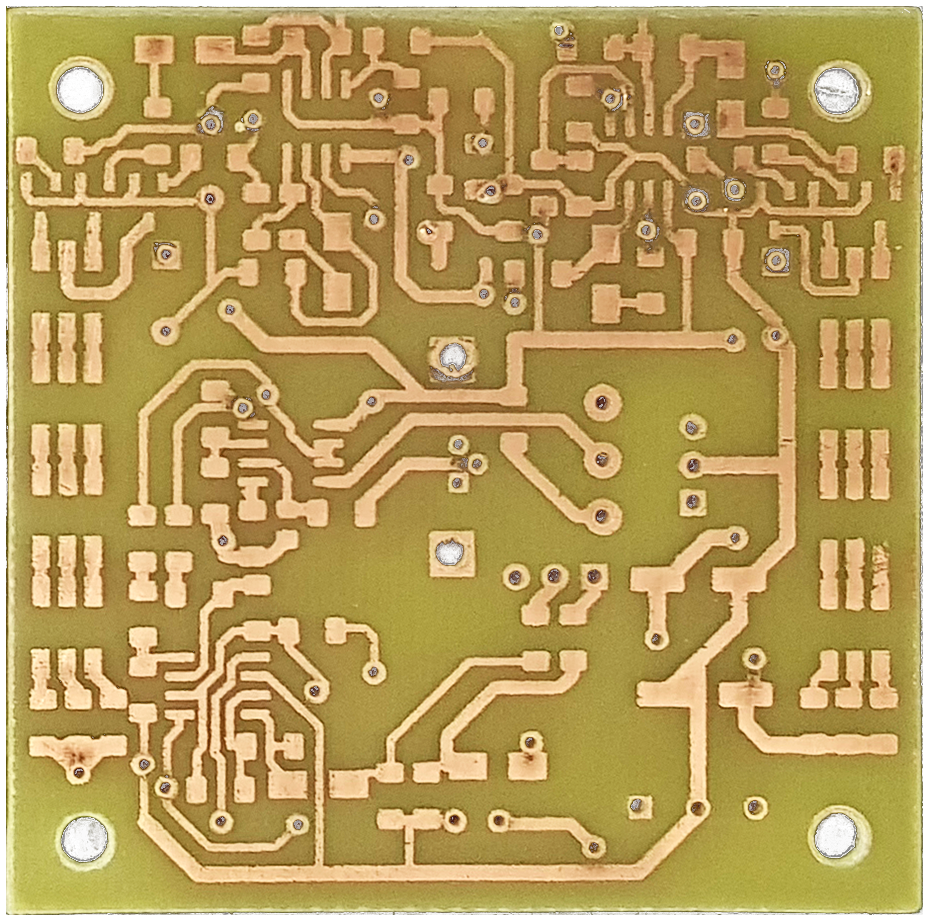
\includegraphics[width=\textwidth]{figures/pcb.png}
    \caption{Printed circuit.}
    \label{}
  \end{subfigure}
  \begin{subfigure}{0.5\textwidth}
    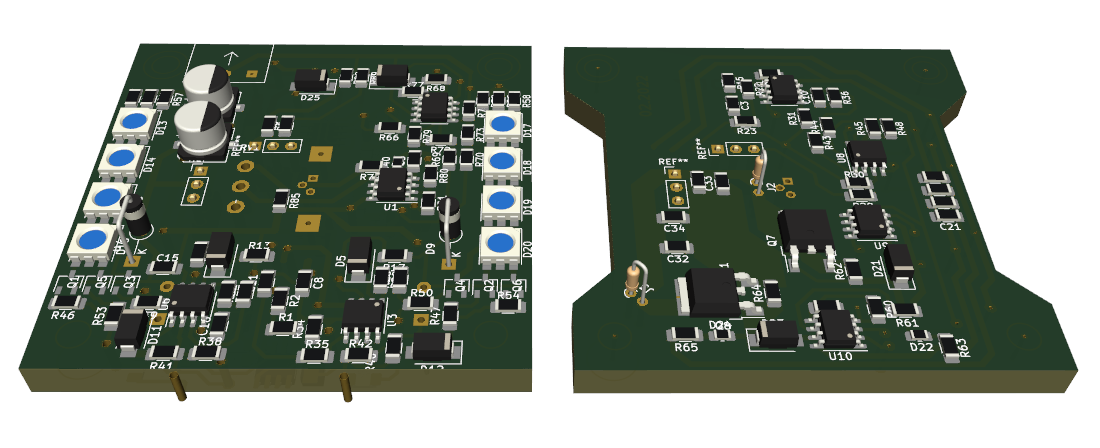
\includegraphics[width=\textwidth]{figures/pcki.png}
    \caption{3D model of the circuit board.}
  \end{subfigure}
  \caption{Digital and manufactured outputs of the PCB.}
\end{figure}



Manufacturing of this PCB is done with copper etching process using basic tools such as laser toner printer, clothes iron and corrosive chemicals. The printouts of the PCB for both boards and layers with processed PCB can be seen in Fig.\ref{PCB}.


\begin{figure}
\centerline{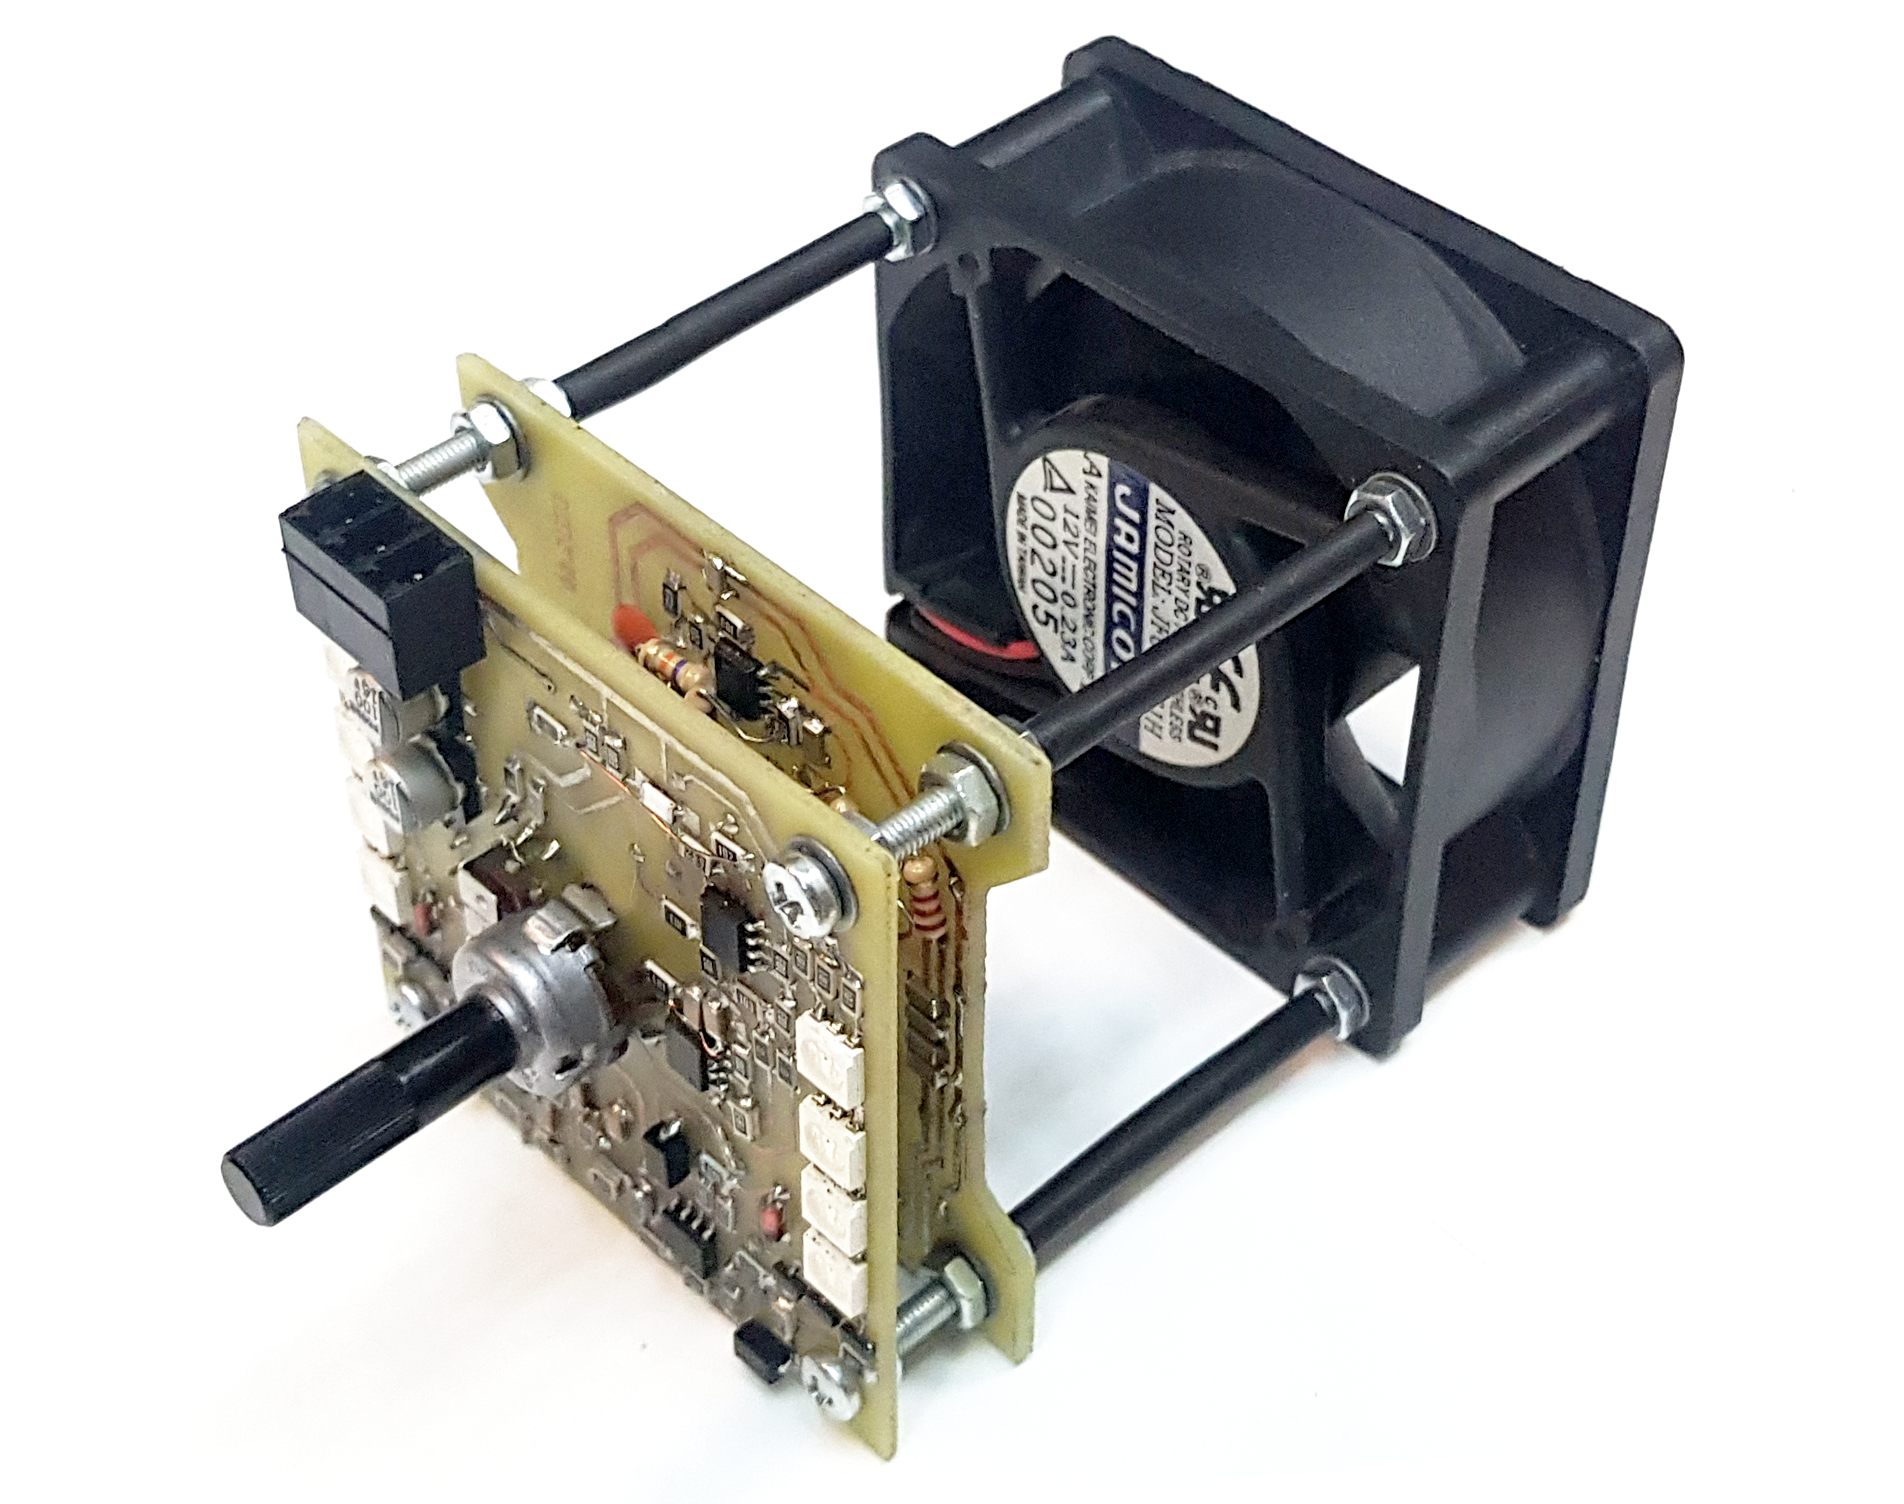
\includegraphics[scale=0.14]{figures/circu.png}}
\caption{Hardware prototype of the designed temperature conditioning system.}
\end{figure}


\section{Thermal Modeling}
This project is composed of two mediums, electrical and thermal. The thermal system consist of heater, fan, temperature sensor and materials in-between. The electrical circuit is as mentioned, consist of the required circuitry to convert the electrical energy to thermal energy. 

In order to simulate the system as a whole it is needed to model the thermal system in electrical analogy. In this analogy, voltage corresponds to the temperature, current corresponds to the heat transfer ratio i.e. power and resistance  corresponds to the thermal resistance. Considering the elements of the thermal system the network is modeled as in Fig. \ref{Thermal}. $R_{\Theta HA}$ is the thermal resistance between the heater and ambient, $R_{\Theta HS}$ is between heater and sensor and $R_{\Theta SA}$ is between sensor and the ambient. The heater is a power controlled current source and the ambient is a fixed voltage source at the room temperature. Lastly the thermal capacitance of the temperature senor is given $C_{sens}$ and nickel-chromium wire is assumed to have very low thermal capacitance while it is very high for the ambient air.

From the datasheet of the LM35 temperature sensor we can find that $R_{\Theta SA}$ is 180 $^\circ C/W$ for the still air. To find the thermal resistance between the heater and the temperature sensor a test is conducted where a known power is applied to the heater and from the temperature difference between the ambient and the sensor with known $R_{\Theta SA}$ the heat flow ratio through the sensor to the ambient is calculated, that is:

\begin{equation}
    \frac{V_{sense}-V_{ambient}}{R_{\Theta SA}}=I_{branch1}
\end{equation}

\begin{equation}
    \frac{V_{heater}-V_{sens}}{I_{branch1}}=R_{\Theta HS}
\end{equation}




\begin{figure}[h]

\centering

\tikzset{every picture/.style={line width=0.75pt}} %set default line width to 0.75pt        

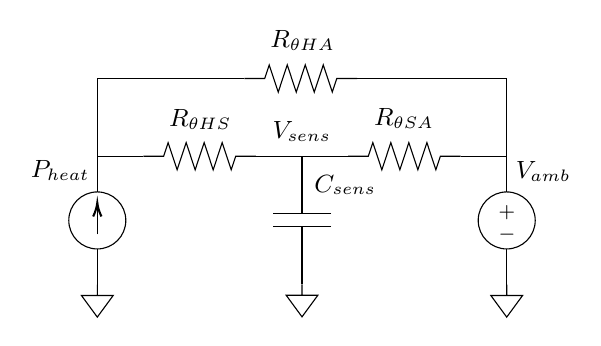
\begin{tikzpicture}[x=0.65pt,y=0.65pt,yscale=-1,xscale=1]
%uncomment if require: \path (0,241); %set diagram left start at 0, and has height of 241

%Shape: Resistor [id:dp19155962871671584] 
\draw   (263,120.55) -- (274.27,120.55) -- (276.77,113) -- (281.78,128.1) -- (286.79,113) -- (291.8,128.1) -- (296.8,113) -- (301.81,128.1) -- (306.82,113) -- (311.83,128.1) -- (314.33,120.55) -- (325.6,120.55) ;
%Shape: Capacitor [id:dp5418351324101072] 
\draw   (351.2,120.55) -- (351.2,152.61) (367.35,159.74) -- (335.05,159.74) (367.35,152.61) -- (335.05,152.61) (351.2,159.74) -- (351.2,191.8) ;
%Straight Lines [id:da2477799830980456] 
\draw    (325.6,120.55) -- (351.2,120.55) ;
%Straight Lines [id:da628273924807907] 
\draw    (351.2,120.55) -- (376.8,120.55) ;
%Shape: Resistor [id:dp5586121261918382] 
\draw   (376.8,120.55) -- (388.07,120.55) -- (390.57,113) -- (395.58,128.1) -- (400.59,113) -- (405.6,128.1) -- (410.6,113) -- (415.61,128.1) -- (420.62,113) -- (425.63,128.1) -- (428.13,120.55) -- (439.4,120.55) ;
%Straight Lines [id:da07949068449386076] 
\draw    (237.4,120.55) -- (263,120.55) ;
%Straight Lines [id:da6123881332149554] 
\draw    (439.4,120.55) -- (465,120.55) ;
%Flowchart: Connector [id:dp3224089439007152] 
\draw   (449.15,156.25) .. controls (449.15,147.5) and (456.25,140.4) .. (465,140.4) .. controls (473.75,140.4) and (480.85,147.5) .. (480.85,156.25) .. controls (480.85,165) and (473.75,172.1) .. (465,172.1) .. controls (456.25,172.1) and (449.15,165) .. (449.15,156.25) -- cycle ;
%Straight Lines [id:da8184153667034564] 
\draw    (465,120.55) -- (465,140.4) ;
%Straight Lines [id:da051595058920608006] 
\draw    (465,172.1) -- (465,191.95) ;
%Straight Lines [id:da6642435742487613] 
\draw    (237.4,120.55) -- (237.4,140.4) ;
%Straight Lines [id:da8967564739142377] 
\draw    (237.4,172.1) -- (237.4,191.95) ;
%Flowchart: Connector [id:dp07363181952530651] 
\draw   (221.55,156.25) .. controls (221.55,147.5) and (228.65,140.4) .. (237.4,140.4) .. controls (246.15,140.4) and (253.25,147.5) .. (253.25,156.25) .. controls (253.25,165) and (246.15,172.1) .. (237.4,172.1) .. controls (228.65,172.1) and (221.55,165) .. (221.55,156.25) -- cycle ;
%Shape: Ground [id:dp6306543326034124] 
\draw   (228.58,197.97) -- (237.4,210) -- (246.23,197.97) -- (228.58,197.97) -- cycle (237.4,191.95) -- (237.4,197.97) ;
%Shape: Ground [id:dp3092481158515603] 
\draw   (342.38,197.82) -- (351.2,209.85) -- (360.03,197.82) -- (342.38,197.82) -- cycle (351.2,191.8) -- (351.2,197.82) ;
%Shape: Ground [id:dp36715519214038794] 
\draw   (456.18,197.97) -- (465,210) -- (473.83,197.97) -- (456.18,197.97) -- cycle (465,191.95) -- (465,197.97) ;
%Straight Lines [id:da5206072269602895] 
\draw    (237.4,164) -- (237.4,148.4) ;
\draw [shift={(237.4,146.4)}, rotate = 90] [color={rgb, 255:red, 0; green, 0; blue, 0 }  ][line width=0.75]    (7.65,-2.3) .. controls (4.86,-0.97) and (2.31,-0.21) .. (0,0) .. controls (2.31,0.21) and (4.86,0.98) .. (7.65,2.3)   ;
%Shape: Resistor [id:dp2796434337397189] 
\draw   (319.2,77.35) -- (330.47,77.35) -- (332.97,69.8) -- (337.98,84.9) -- (342.99,69.8) -- (348,84.9) -- (353,69.8) -- (358.01,84.9) -- (363.02,69.8) -- (368.03,84.9) -- (370.53,77.35) -- (381.8,77.35) ;
%Straight Lines [id:da12366662536381101] 
\draw    (237.4,124.7) -- (237.4,77.35) ;
%Straight Lines [id:da01760570202550582] 
\draw    (237.4,77.35) -- (319.2,77.35) ;
%Straight Lines [id:da3751939511907125] 
\draw    (465,124.7) -- (465,77.35) ;
%Straight Lines [id:da29961110180248873] 
\draw    (381.8,77.35) -- (465,77.35) ;

% Text Node
\draw (451.2,144.4) node [anchor=north west][inner sep=0.75pt]  [font=\scriptsize]  {$ \begin{array}{l}
\mathbf{{\displaystyle +}}\\
\mathbf{{\displaystyle -}}
\end{array}$};
% Text Node
\draw (468.6,122.2) node [anchor=north west][inner sep=0.75pt]  [font=\small]  {$V_{amb}$};
% Text Node
\draw (389.8,92.4) node [anchor=north west][inner sep=0.75pt]  [font=\small]  {$R_{\theta SA}$};
% Text Node
\draw (275.8,93.2) node [anchor=north west][inner sep=0.75pt]  [font=\small]  {$R_{\theta HS}$};
% Text Node
\draw (332.2,49.4) node [anchor=north west][inner sep=0.75pt]  [font=\small]  {$R_{\theta HA}$};
% Text Node
\draw (199,121.4) node [anchor=north west][inner sep=0.75pt]  [font=\small]  {$P_{heat}$};
% Text Node
\draw (333.4,99.8) node [anchor=north west][inner sep=0.75pt]  [font=\small]  {$V_{sens}$};
% Text Node
\draw (356.6,129.6) node [anchor=north west][inner sep=0.75pt]  [font=\small]  {$C_{sens}$};


\end{tikzpicture}
\caption{Thermal network model using the electrical circuit elements}
\label{Thermal}
\end{figure}

Later the thermal resistance between the heater and the ambient can be found using again the same technique. Rest of the power flows through the branch 2, that is the upper branch.


\begin{equation}
    I_{power}-I_{branch1}=I_{branch2}
\end{equation}

\begin{equation}
    \frac{V_{heater}-V_{ambient}}{I_{branch2}}=R_{\Theta HA}
\end{equation}

A test voltage of 3.5V is applied to the heater and 0.56 ampere of current is passed resulting in 1.96 watts of power is dissipated on the resistor. From (6) thermal current on branch1 is 0.2033W and on branch2 it is 1.757W. At this stage nickel-chromium wire heated up to 131.5 $\celsius$. Steady state test shows that $R_{\Theta HS}$ is 650 $\celsius$/W, $R_{\Theta HA}$ is 62 $\celsius$/W.

Transient test is applied in order to measure the thermal capacitance. The time constant of the thermal circuit is measured with heating cycle of the system and $C_{sense}$ is measured to be 172 millifarads.

The last test applied in order to fully model the system is the cooling test.The fan effectively reduces the thermal resistance between the temperature sensor and the ambient temperature. For the test the fan is turned on and steady state values of the thermal resistances are measured with constant air flow over the system. Assuming the exiting air velocity is proportional with the motor speed in operation region andair velocity and the convection ratio of the system is in linear relation the thermal resistances are modeled as such\eqref{term}.

\begin{equation}
    R_{\Theta SA}=180-V_{fan}*12
    \label{term}
\end{equation}

\section{Simulation Results}

There are three critical specifications about this project that one can simulate. The first one is that the set and ambient display LEDs must cover the light spectrum with a smooth transition while the set and ambient temperatures cover the whole temperature range (24-40\celsius). The second one is that the fan and the resistor should never act at the same time. Finally, the control and the operation units work effective enough so that the temperature is adjusted rapidly and accurately. The simulations are done on LTspice, the data are exported and plotted in MATLAB. 

To show that the LED currents are as desired, a ramp input is given instead of the temperature measurement to the display unit, and the LED currents are observed in the simulation. Observed current signals are plotted in Fig.~\ref{displaySweep}, which is very close to the desired current signals in Fig.~\ref{ILED}

\begin{figure}
\centerline{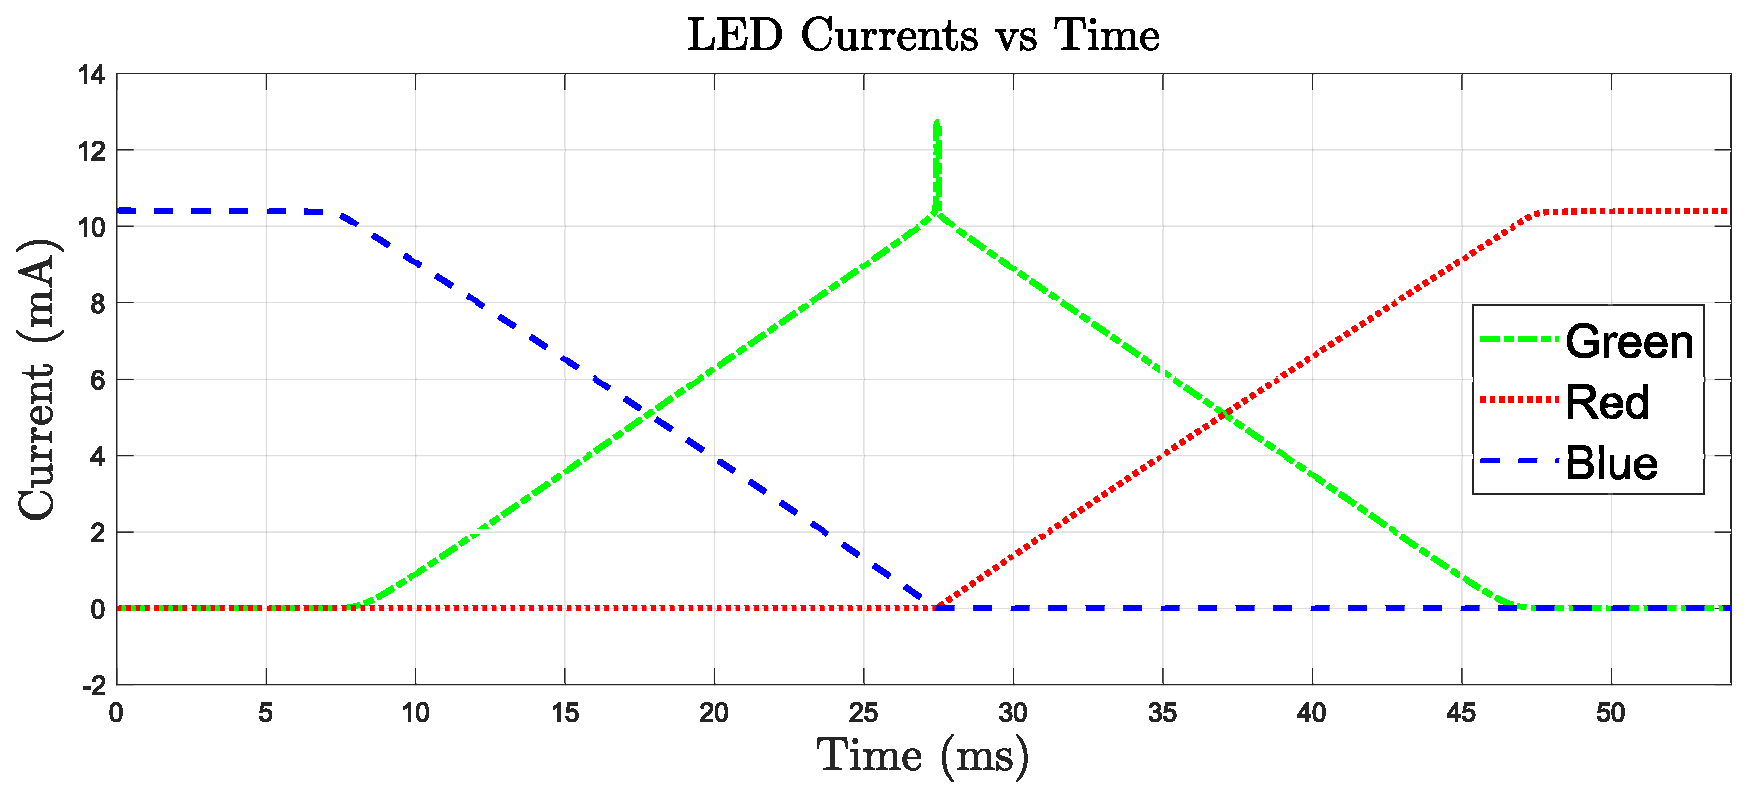
\includegraphics[scale=0.31]{figures/displaySweep.eps}}
\caption{Simulated LED currents vs time graphs for each color terminal}
\label{displaySweep}
\end{figure}

To show the other specifications are satisfied, it is needed to model the whole system in LTspice (including the thermal circuit in Fig.~\ref{Thermal}). Fig.~\ref{pwmSim} includes the PWM signals produced for the heater and the fan together. Since they do not intersect, it is concluded that the comparator works as desired.

\begin{figure}
\centerline{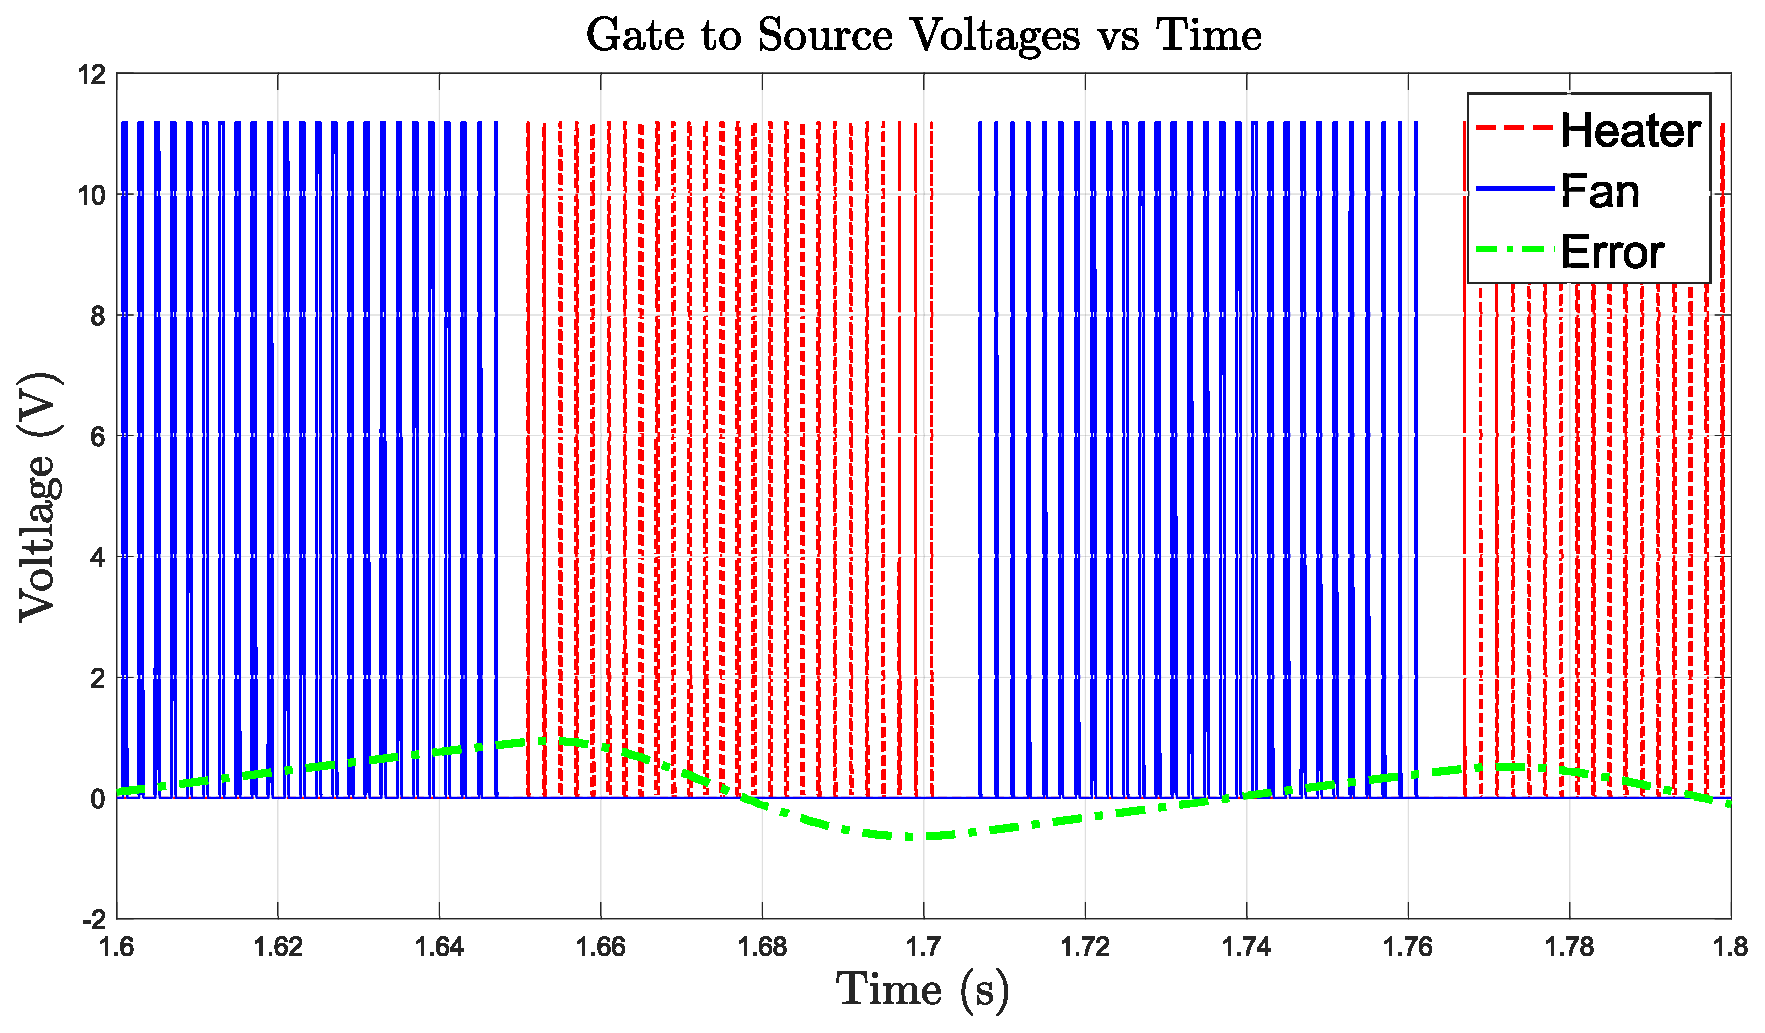
\includegraphics[scale=0.31]{figures/pwmsim.eps}}
\caption{Simulated PWM signals for the heater and the fan}
\label{pwmSim}
\end{figure}

Using the same model, Fig.~\ref{pidSim} includes the set and the ambient temperature value waveforms. One can see from Fig.~\ref{pidSim} that the PID controller is able to reduce the error to a desired margin in a reasonable time for our model. Note that this simulation result is only a proof-of-concept showing that PID controller will work in the designed model. The tuning should be done experimentally.

\begin{figure}
\centerline{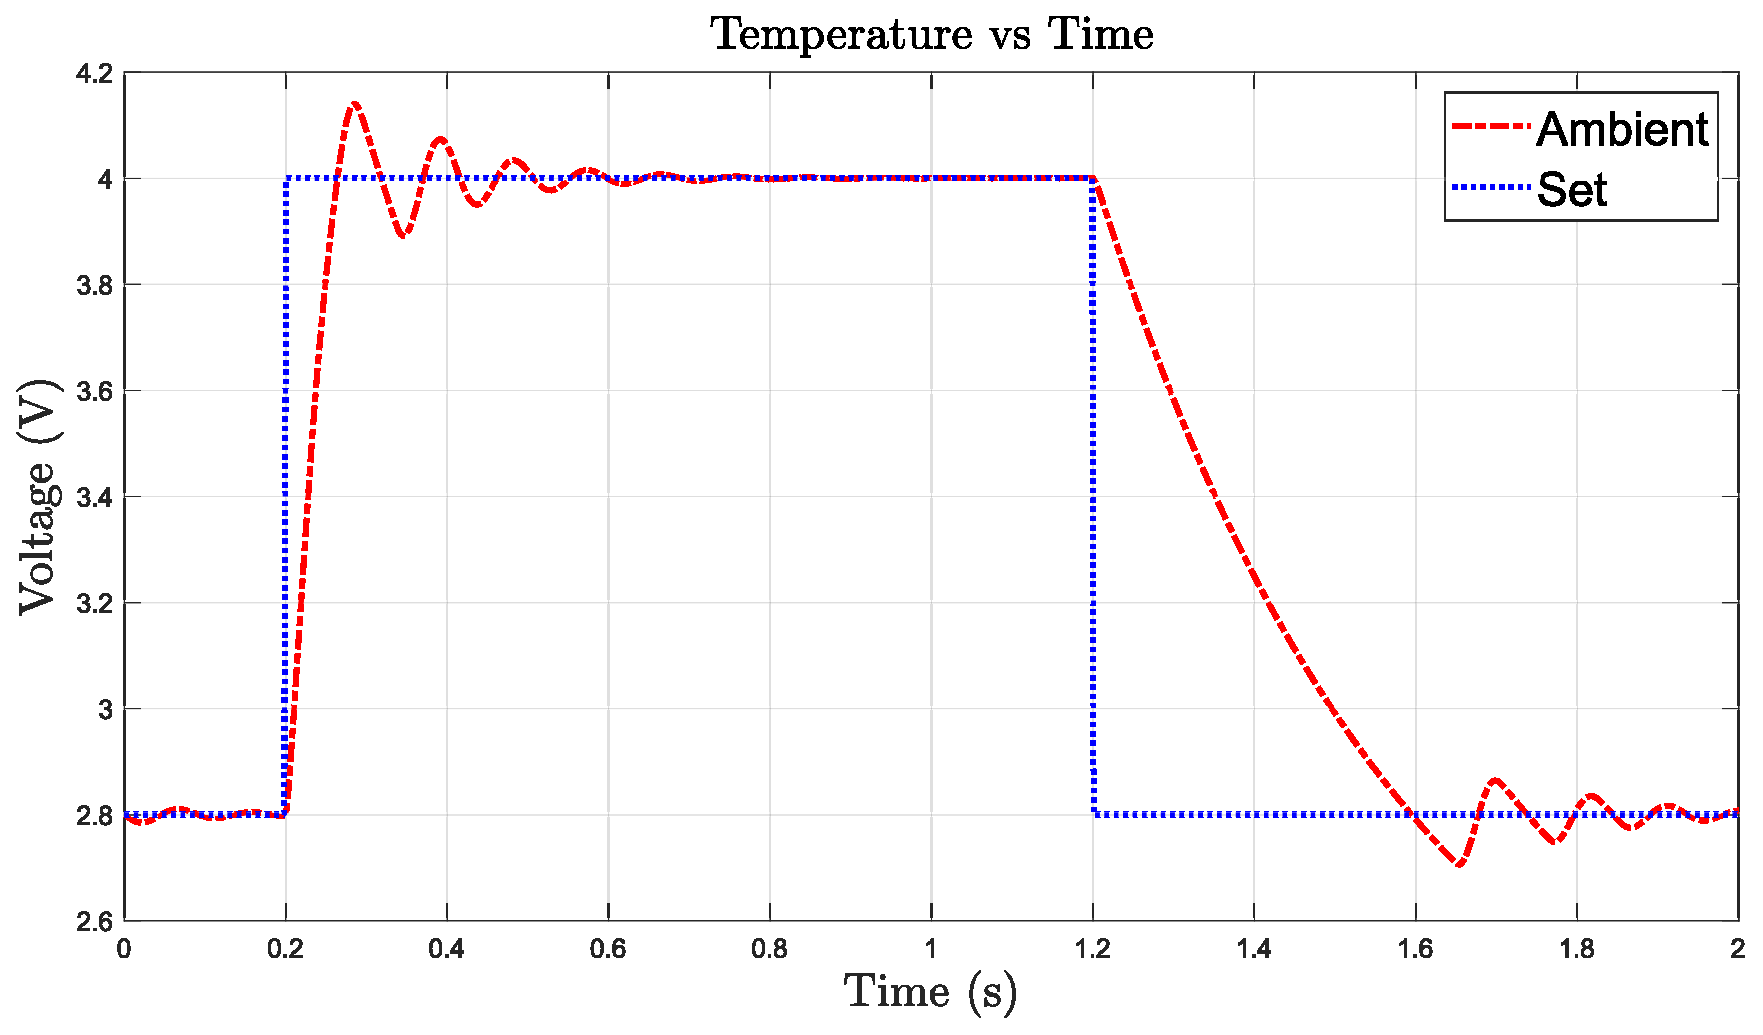
\includegraphics[scale=0.31]{figures/pidsim.eps}}
\caption{Simulated set and ambient temperature signals over time}
\label{pidSim}
\end{figure}


\section{Experimental Results}

In the first experiment, the base emitter voltages of the BJTs are measured using an oscilloscope. The results were consistent with the simulation results as expected. The transition was smooth and covering all the range.

In the second experiment, the set and the ambient temperature values are observed on the oscilloscope screen and the data is plotted in Fig.~\ref{pidRise} and Fig.~\ref{pidFall}. One can see that the full temperature can be adjusted and settled to a value very rapidly and accurately. The settling time is around 15 seconds, and the steady state error is strictly less than 1\celsius. As expected from the theoretical knowledge and simulation results, PID method works brilliantly in this specific case.

\begin{figure}
\centerline{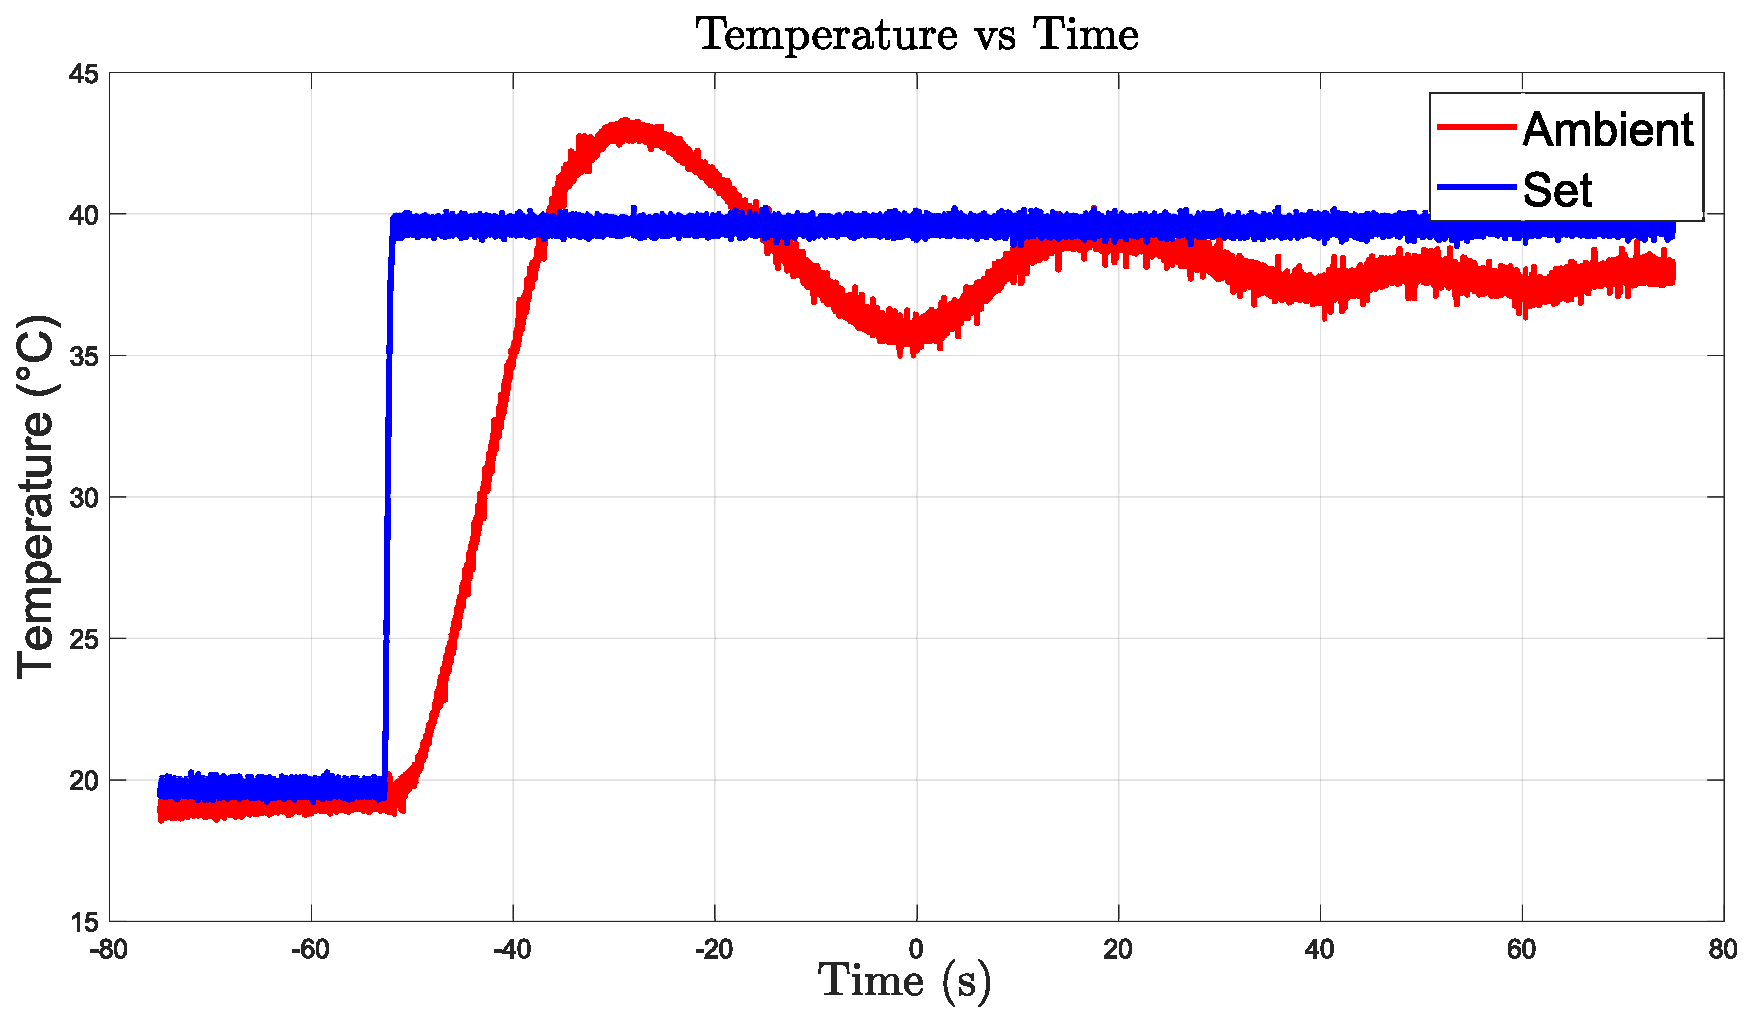
\includegraphics[scale=0.31]{figures/pidRise.eps}}
\caption{Experimental set and ambient temperature signals (rise)}
\label{pidRise}
\end{figure}

\begin{figure}
\centerline{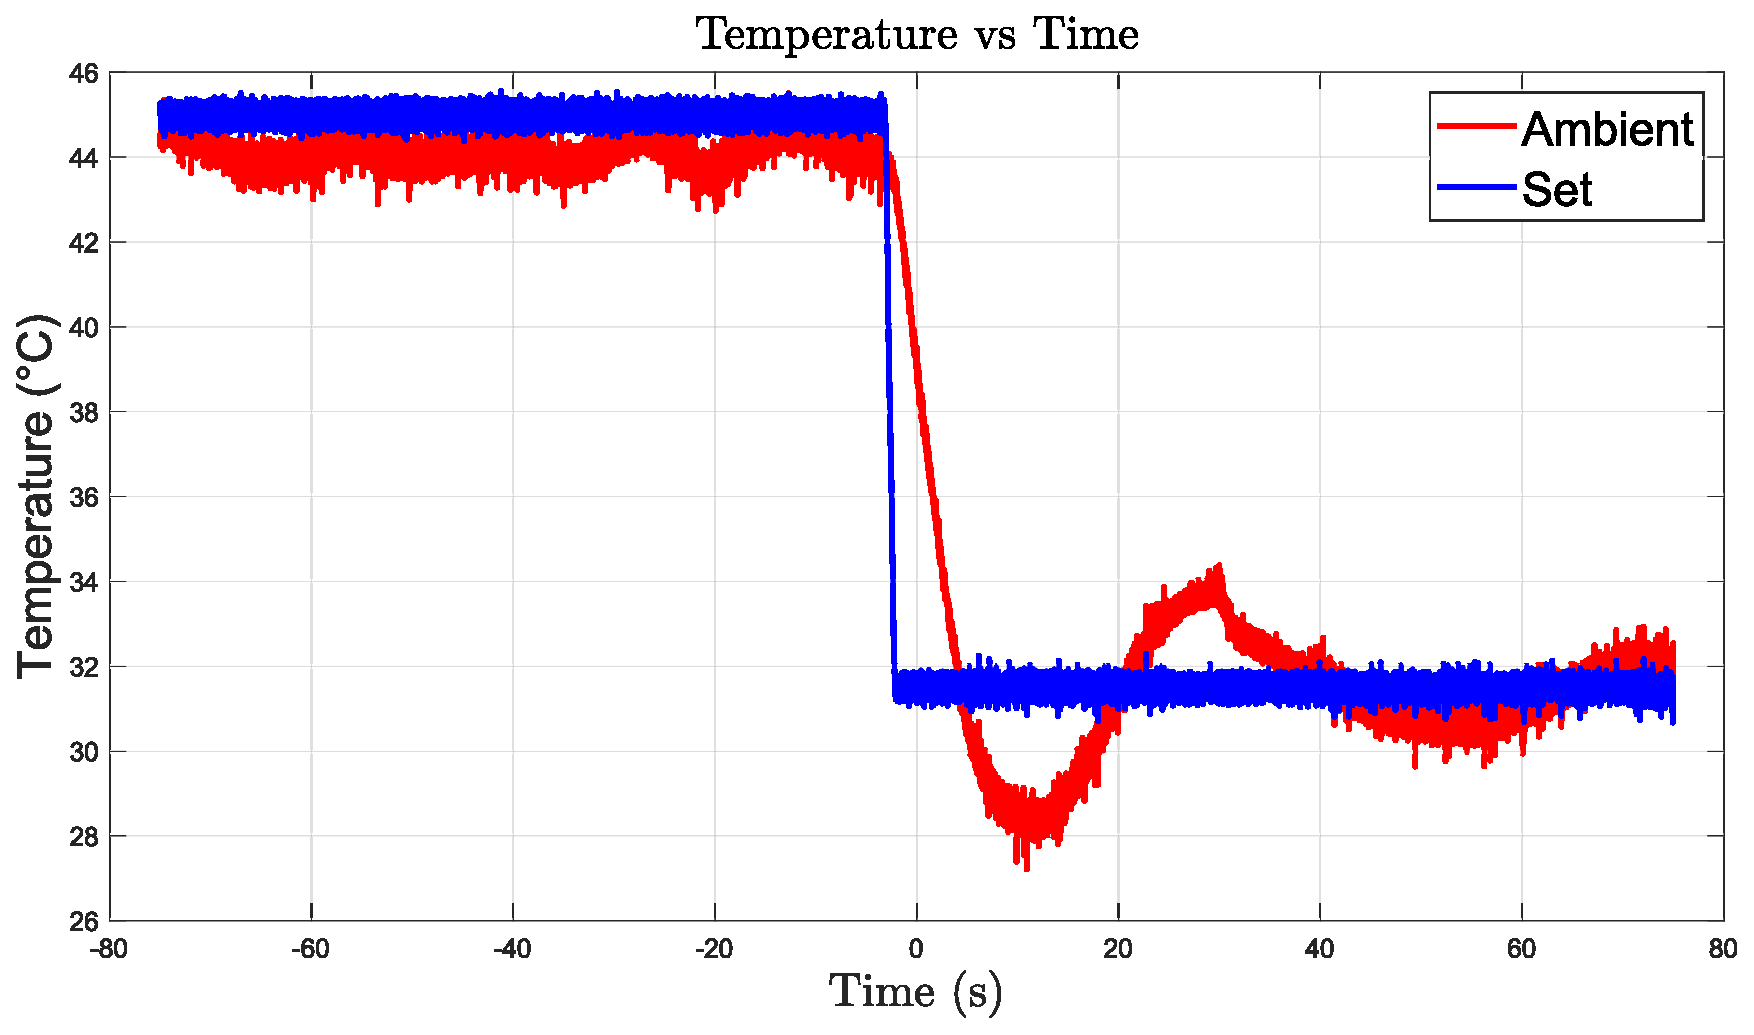
\includegraphics[scale=0.31]{figures/pidFall.eps}}
\caption{Experimental set and ambient temperature signals (fall)}
\label{pidFall}
\end{figure}

There are no detectable discrepancies with the theoretical and the simulation results, which means the accuracy of the models that are used are very high. Even if there are some deviations, they may be due to the non-idealities of the components and thermal disturbances.

\section{Conclusions}
In this paper, the design and implementation of an autonomous temperature conditioning system is demonstrated. Electrical and thermal systems are modelled in a single simulation environment with feedback loop closed. The PID method is shown that its applicable to this system, but due to the asymmetry of the reverse processes a modified PID circuit is proposed to damp oscillations of the system around the steady state, which is shown to be successful with the experimental results. Moreover, since the control signals are critical for the process, it is observed that filtering the noise with low and high pass filters and also avoiding the EMI effects with a careful PCB design procedure is essential for an accurate and reliable control mechanism.


\begin{thebibliography}{00}
\bibitem{b1} Y. Wu, J. P. Bobis and R. Gehman, "The design and analysis of an improved high air flow meter with analog/digital filters," [1992] Conference Record IEEE Instrumentation and Measurement Technology Conference, 1992, pp. 600-605, doi: 10.1109/IMTC.1992.245068.

\bibitem{b2}Kiam Heong Ang, G. Chong and Yun Li, "PID control system analysis, design, and technology," in IEEE Transactions on Control Systems Technology, vol. 13, no. 4, pp. 559-576, July 2005, doi: 10.1109/TCST.2005.847331.

\bibitem{b3}A. Baskys and V. Zlosnikas, "Asymmetric PID controller," IECON 2006 - 32nd Annual Conference on IEEE Industrial Electronics, 2006, pp. 219-223, doi: 10.1109/IECON.2006.347936.

\bibitem{b4} A. A. Kilov, V. N. Konstantyan, A. S. Sannikov, S. A. Sheptunov and A. A. Chetvertakov, "Applying Digital Filters to Suppress Noise in the Derivative Term of the PID Controller," 2021 International Conference on Quality Management, Transport and Information Security, Information Technologies (IT&QM&IS), 2021, pp. 301-304, doi: 10.1109/ITQMIS53292.2021.9642889.



\end{thebibliography}
\end{document}
